\section{Proposed KDS-EL Algorithm}\label{sec:proposed}

In this section, we present the comprehensive architectural design, mathematical formulation, and algorithmic execution of the proposed \textbf{Knowledge-Guided Dual-Phase Swarm Evolutionary Learning (KDS-EL)} algorithm. KDS-EL is designed specifically to overcome three fundamental structural deficiencies of conventional particle swarm optimization in ultra-high-dimensional feature selection: (i) the search inefficiency and wasted evaluation budget caused by uniform random initialization in sparse feature spaces, (ii) the loss of historical cross-iteration feature-importance signals due to memoryless random perturbation, and (iii) the inability of static objective weighting to adapt to the divergent requirements of coarse feature reduction versus fine-grained accuracy refinement.

\subsection{Overall Algorithmic Architecture}

\begin{figure}[!htb]
\centering
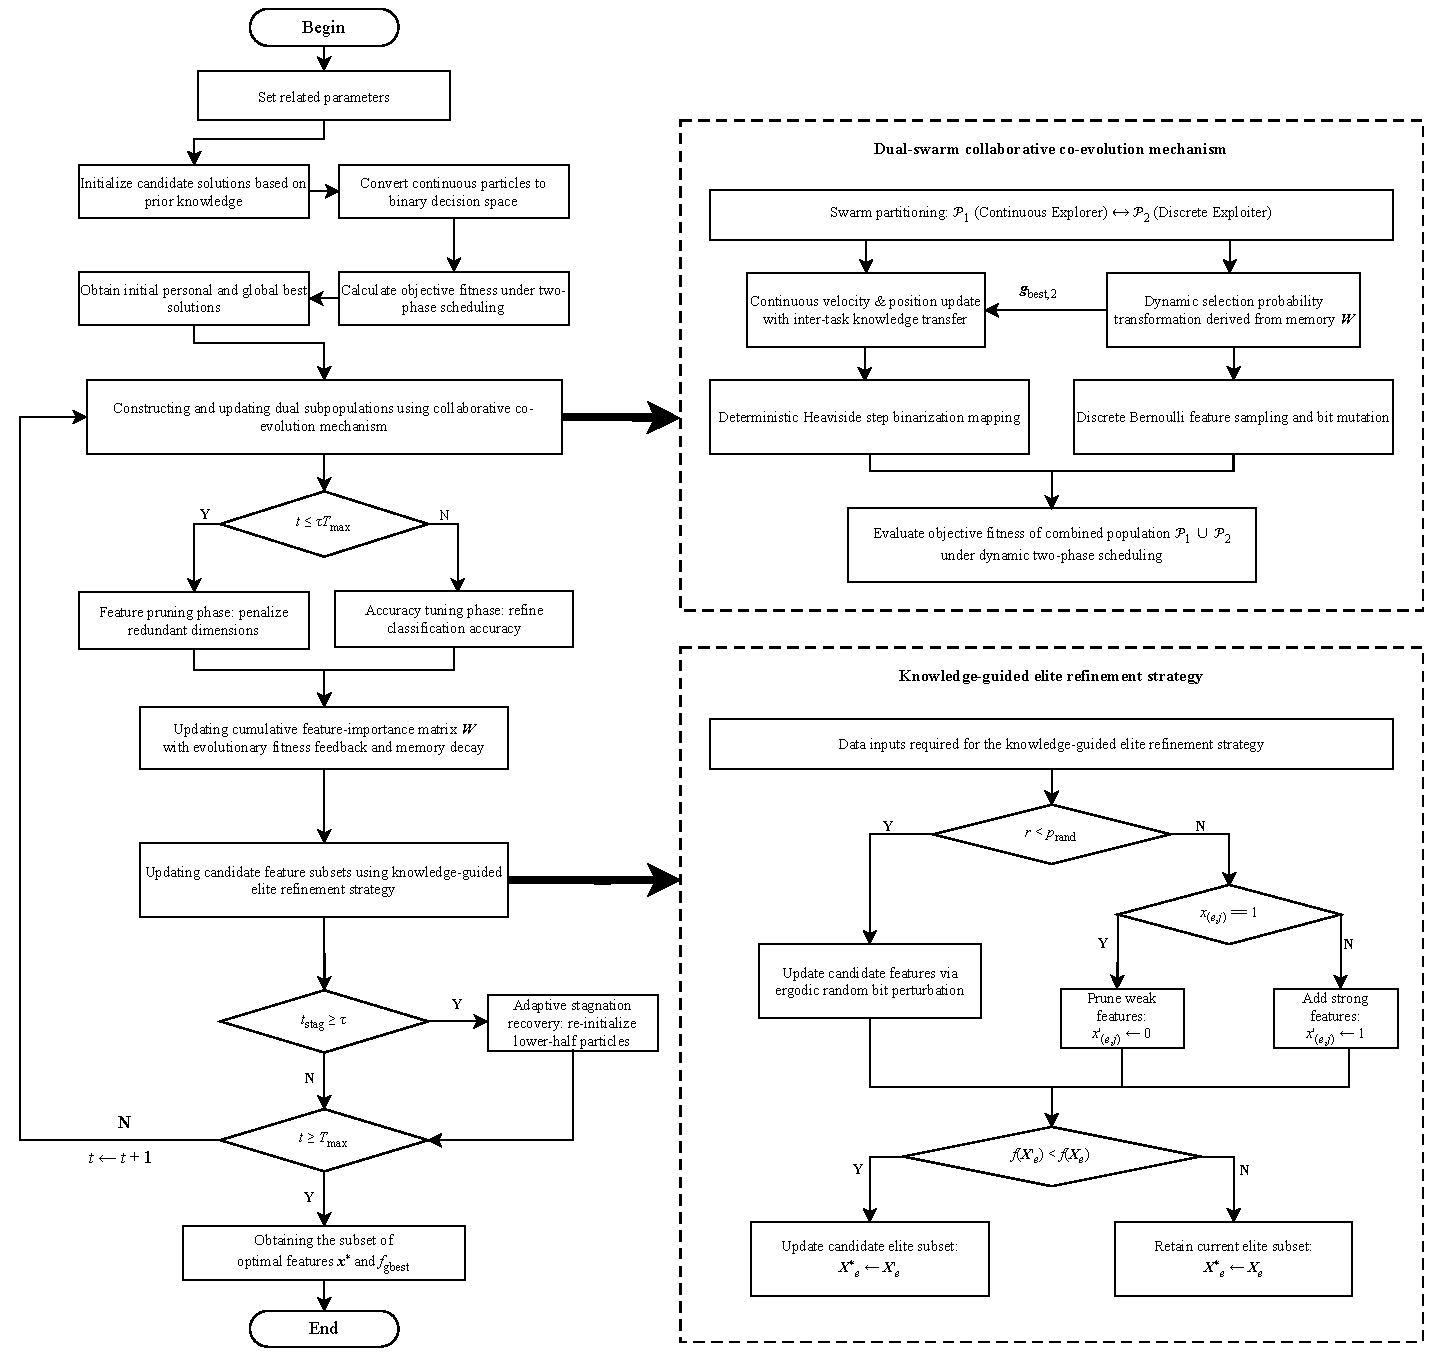
\includegraphics[width=\linewidth]{F1_architecture_journal.pdf}
\caption{Overall architectural pipeline of KDS-EL: high-dimensional data undergo filter-based mutual information ranking, dual-subpopulation initialization with Gaussian perturbation, two-phase dynamic objective weight scheduling, cross-iteration cumulative feature-importance matrix accumulation with exponential decay, and knowledge-guided elite refinement with 1-to-1 in-place replacement.}
\label{F1}
\end{figure}

The macroscopic architecture of KDS-EL is illustrated in Fig.~\ref{F1}. Built upon a cooperative multi-task dual-subpopulation backbone~\cite{mel2024}, KDS-EL divides a population of $N=20$ binary particles into two collaborative subpopulations of equal size ($N_1 = N_2 = 10$). Subpopulation~1 ($\mathcal{P}_1$) executes standard continuous-space PSO velocity-position updates with an inter-task knowledge transfer channel directing particles toward the historical global best of Subpopulation~2. Subpopulation~2 ($\mathcal{P}_2$) performs probability-driven feature sampling guided by the population's accumulated feature-importance landscape.

The optimization process operates in a closed loop through four tightly coupled functional stages:
\begin{enumerate}
    \item \textbf{Filter-Level Quality Bootstrapping (Offline)}: Mutual information (MI) between each feature and class labels is computed once prior to evolution, establishing a normalized baseline relevance vector $\mathbf{m} \in [0, 1]^D$.
    \item \textbf{Knowledge-Informed Hybrid Seeding}: An initial population of $N$ particles is generated by blending Gaussian-perturbed MI seeds with uniform random particles at a ratio of $\mathrm{MI\_init\_ratio}=0.50$, followed by Heaviside step binarization with threshold $\theta=0.60$.
    \item \textbf{Dynamic Two-Phase Evolutionary Loop}: Across $T=100$ iterations, the objective weights $\mathbf{w}(t) = [w_a(t), w_f(t)]$ dynamically transition from aggressive feature pruning ($\mathbf{w}_1 = [0.70, 0.30]$ for $t \le 0.7T$) to accuracy-oriented refinement ($\mathbf{w}_2 = [0.95, 0.05]$ for $t > 0.7T$).
    \item \textbf{Accumulative Knowledge Harvesting and Elite Refinement}: Fitness improvements during evaluation are harvested into a continuous feature-importance matrix $W \in \mathbb{R}^D$, discounted by an exponential forgetting factor $\gamma=0.99$. The top $\mathrm{elite\_k}=3$ elite individuals are refined via the Knowledge-guided Elite Refinement (KER) operator and admitted via 1-to-1 in-place replacement. An adaptive re-initialization mechanism monitors stagnation and re-seeds the lower half of the population if global-best fitness stalls for $\mathrm{stall\_patience}=20$ generations.
\end{enumerate}

\subsection{MI-Prior Seeding and Adaptive Re-injection Strategy}\label{sec:mi}

\subsubsection{Deficiency Analysis and Design Rationale}

Standard binary meta-heuristics universally initialize particle positions via uniform random sampling over $[0, 1]^D$. In an ultra-high-dimensional feature space where $D \gg 10^3$, uniform random initialization produces candidate solutions where approximately $50\%$ of all features are active ($\|\mathbf{x}\|_0 \approx D/2$). However, for biomedical classification problems, true informative biomarker subsets are notoriously sparse, typically comprising fewer than $100$ genes ($\|\mathbf{x}^{\star}\|_0 \ll 0.01 D$). Consequently, random initialization forces the swarm into dense, highly redundant, and noisy search basins, squandering a major fraction of the computational evaluation budget simply attempting to discard thousands of irrelevant features.

To resolve this initial cold-start inefficiency, KDS-EL establishes a filter-wrapper hybrid seeding strategy that injects prior feature-relevance knowledge into the swarm origin while preserving sufficient stochastic diversity.

\subsubsection{Mathematical Formulation of MI Seeding}

Let $\mathcal{D} = \{(\mathbf{f}_i, y_i)\}_{i=1}^{N_{\mathrm{samp}}}$ denote the training set with $D$-dimensional feature vectors $\mathbf{f}_i$ and class labels $y_i \in \{1, \ldots, C\}$. The mutual information $I(f_j; Y)$ between the $j$-th feature $f_j$ and the label $Y$ is defined as:
\begin{equation}
I(f_j; Y) = \sum_{v \in \mathrm{Val}(f_j)} \sum_{c = 1}^C P(f_j = v, Y = c) \log_2 \frac{P(f_j = v, Y = c)}{P(f_j = v) P(Y = c)}.
\label{eq:mi_def}
\end{equation}
The continuous feature values are discretized into equal-frequency bins to estimate probability distributions. The raw MI scores $\{I(f_j; Y)\}_{j=1}^D$ are normalized into a baseline relevance vector $\mathbf{m} \in [0, 1]^D$:
\begin{equation}
m_j = \frac{I(f_j; Y) - \min_{1 \le k \le D} I(f_k; Y)}{\max_{1 \le k \le D} I(f_k; Y) - \min_{1 \le k \le D} I(f_k; Y) + \epsilon},
\label{eq:mi_norm}
\end{equation}
where $\epsilon = 10^{-12}$ prevents division by zero.

\begin{figure*}[!htb]
\centering
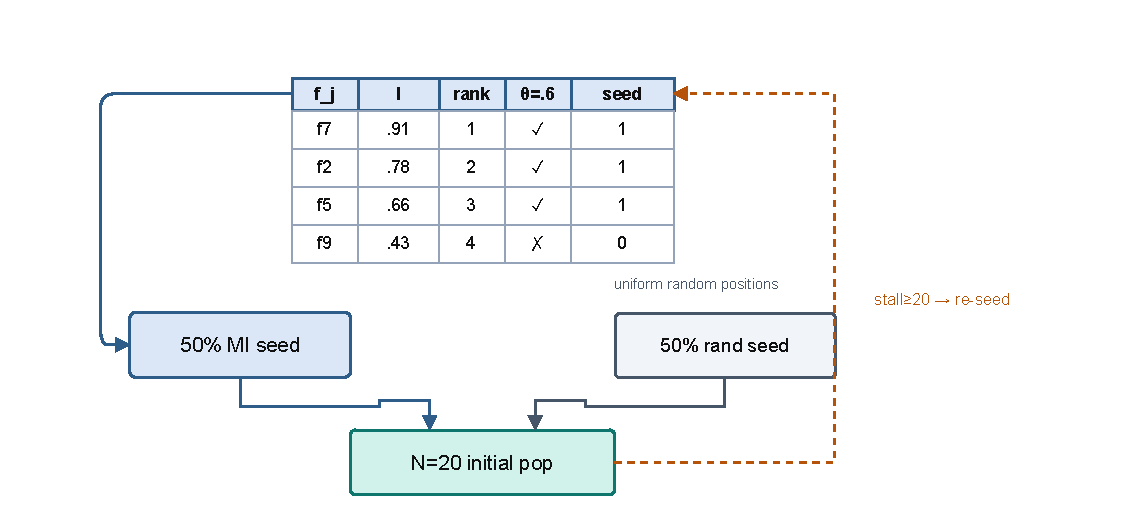
\includegraphics[width=0.96\linewidth]{F2_mi_initialization_journal.pdf}
\caption{Operational mechanism of MI-Prior Seeding and Adaptive Re-injection: mutual information $I(f_j; \mathbf{Y})$ extracts continuous feature--target dependency to construct a normalized prior vector $\widetilde{\mathbf{m}} \in [0, 1]^D$, which biases $50\%$ of initial particles with Gaussian perturbation while the remaining $50\%$ undergo uniform random exploration; when evolutionary search encounters stagnation ($\mathrm{stall} \ge 20$), the MI prior is adaptively re-injected into inferior particles to restore search vitality.}
\label{F2}
\end{figure*}

To prevent population homogenization while guiding search toward informative dimensions, the initial population is split into two halves based on $\rho = \mathrm{MI\_init\_ratio} = 0.50$:
\begin{equation}
\mathbf{p}_i = \begin{cases}
\mathrm{clip}\bigl(\mathbf{m} + \boldsymbol{\varepsilon}_i, \; 0, \; 1\bigr), \quad \boldsymbol{\varepsilon}_i \sim \mathcal{N}(\mathbf{0}, \sigma^2 I_D), & \text{for } 1 \le i \le \rho N,\\[4pt]
\mathbf{u}_i, \quad \mathbf{u}_i \sim \mathcal{U}(0, 1)^D, & \text{for } \rho N < i \le N,
\end{cases}
\label{eq:mi_seeding}
\end{equation}
where $\sigma = 0.10$ represents the Gaussian noise perturbation scale and $\mathrm{clip}(z, 0, 1) = \max(0, \min(1, z))$.

Continuous positions $\mathbf{p}_i = [p_{i,1}, \ldots, p_{i,D}]$ are mapped into binary feature selection vectors $\mathbf{x}_i \in \{0, 1\}^D$ using a strict Heaviside step binarization with threshold $\theta = 0.60$:
\begin{equation}
x_{i,j} = \begin{cases}
1, & \text{if } p_{i,j} \ge \theta,\\[2pt]
0, & \text{if } p_{i,j} < \theta.
\end{cases}
\label{eq:binarize}
\end{equation}
Because $\theta = 0.60 > 0.50$, only features possessing above-average mutual information are initialized as active, naturally yielding a sparse initial configuration ($\|\mathbf{x}_i\|_0 \approx 0.15 D \sim 0.30 D$) that accelerates early convergence. Algorithm~\ref{alg:mi_init} specifies the hybrid initialization procedure.

\begin{algorithm}[!htb]
\caption{MI-Guided Population Initialization}
\label{alg:mi_init}
\begin{algorithmic}[1]
\Require Normalized MI score vector $\mathbf{m} \in [0, 1]^D$, population size $N=20$, seeding ratio $\rho=0.50$, threshold $\theta=0.60$, noise scale $\sigma=0.10$
\Ensure Hybrid binary initial population $\mathcal{P} = \{\mathbf{x}_i\}_{i=1}^N$ and continuous positions $\{\mathbf{p}_i\}_{i=1}^N$
\For{$i = 1$ \textbf{to} $N$}
    \If{$i \le \lfloor \rho N \rfloor$}
        \State Sample perturbation $\boldsymbol{\varepsilon}_i \sim \mathcal{N}(\mathbf{0}, \sigma^2 I_D)$
        \State $\mathbf{p}_i \leftarrow \max\bigl(\mathbf{0}, \min(\mathbf{1}, \mathbf{m} + \boldsymbol{\varepsilon}_i)\bigr)$ \Comment{Knowledge-guided continuous seed}
    \Else
        \State Sample continuous position $\mathbf{p}_i \sim \mathcal{U}(0, 1)^D$ \Comment{Random exploratory seed}
    \EndIf
    \For{$j = 1$ \textbf{to} $D$}
        \State $x_{i,j} \leftarrow \mathbb{I}(p_{i,j} \ge \theta)$ \Comment{Thresholded binarization \eqref{eq:binarize}}
    \EndFor
\EndFor
\State \Return Binary population $\{\mathbf{x}_i\}_{i=1}^N$ and continuous positions $\{\mathbf{p}_i\}_{i=1}^N$
\end{algorithmic}
\end{algorithm}

\subsubsection{Adaptive Stagnation Re-initialization}

High-dimensional multimodal search landscapes frequently cause swarm particles to become trapped in suboptimal local attractors. When the global-best fitness $f_{\mathrm{gbest}}$ fails to improve for $\tau = \mathrm{stall\_patience} = 20$ consecutive iterations, an adaptive re-initialization routine is triggered:
\begin{enumerate}
    \item The population is sorted in ascending order of personal-best fitness $f_i^{\mathrm{pbest}}$.
    \item The superior half ($\{i \mid \mathrm{rank}(i) \le N/2\}$) is preserved to safeguard historical elite trajectories.
    \item The inferior half ($\{i \mid \mathrm{rank}(i) > N/2\}$) is fully refreshed using the Gaussian-perturbed MI distribution:
    \begin{equation}
    \mathbf{p}_i \leftarrow \mathrm{clip}\bigl(\mathbf{m} + \boldsymbol{\varepsilon}_i, \; 0, \; 1\bigr), \quad x_{i,j} \leftarrow \mathbb{I}(p_{i,j} \ge \theta).
    \label{eq:reinit_formula}
    \end{equation}
    \item The refreshed particles are re-evaluated under the current objective weights, and the stagnation counter is reset to zero.
\end{enumerate}
This restores diversity within a high-potential subspace without completely discarding established elite knowledge, as formalized in Algorithm~\ref{alg:mi_reinit}.

\begin{algorithm}[!htb]
\caption{Adaptive Stagnation Re-initialization}
\label{alg:mi_reinit}
\begin{algorithmic}[1]
\Require Population $\{\mathbf{x}_i, \mathbf{p}_i\}_{i=1}^N$, personal bests $\{\mathbf{p}_{\mathrm{best},i}, f_i^{\mathrm{pbest}}\}_{i=1}^N$, MI vector $\mathbf{m}$, threshold $\theta=0.60$, noise scale $\sigma=0.10$, objective weights $\mathbf{w}(t)$
\Ensure Refreshed population $\mathcal{P}$ with restored swarm diversity
\State Sort population indices $\pi$ such that $f_{\pi(1)}^{\mathrm{pbest}} \le f_{\pi(2)}^{\mathrm{pbest}} \le \cdots \le f_{\pi(N)}^{\mathrm{pbest}}$
\For{$k = \lfloor N/2 \rfloor + 1$ \textbf{to} $N$}
    \State $i \leftarrow \pi(k)$ \Comment{Target inferior particle}
    \State Sample perturbation $\boldsymbol{\varepsilon}_i \sim \mathcal{N}(\mathbf{0}, \sigma^2 I_D)$
    \State $\mathbf{p}_i \leftarrow \max\bigl(\mathbf{0}, \min(\mathbf{1}, \mathbf{m} + \boldsymbol{\varepsilon}_i)\bigr)$
    \State $x_{i,j} \leftarrow \mathbb{I}(p_{i,j} \ge \theta), \quad \forall j \in \{1, \ldots, D\}$
    \State Evaluate fitness $f_i \leftarrow f(\mathbf{x}_i, \mathbf{w}(t))$ using \eqref{eq:fitness}
    \State $\mathbf{p}_{\mathrm{best},i} \leftarrow \mathbf{x}_i, \quad f_i^{\mathrm{pbest}} \leftarrow f_i$
\EndFor
\State \Return Updated population and personal bests
\end{algorithmic}
\end{algorithm}

\subsection{Cumulative Feature-Importance Matrix with Exponential Memory Decay}\label{sec:importance}

\subsubsection{Deficiency Analysis and Design Rationale}

Standard PSO operators update particle trajectories purely based on instantaneous personal best ($\mathbf{p}_{\mathrm{best}}$) and global best ($\mathbf{g}_{\mathrm{best}}$) coordinates. Across consecutive evolutionary cycles, thousands of candidate subset evaluations are performed, generating abundant empirical evidence regarding which specific feature additions or deletions consistently enhance classification performance. Standard meta-heuristics completely discard this trial-and-error feedback upon the conclusion of each generation, suffering from severe evolutionary memory loss.

To capture and retain this cross-iteration evolutionary feedback, KDS-EL maintains a global continuous \textbf{Cumulative Feature-Importance Matrix} $W \in \mathbb{R}^D$, initialized to the zero vector $\mathbf{0}$.

\subsubsection{Differential Feedback Update and Exponential Forgetting}

At generation $t$, whenever a newly evaluated particle $\mathbf{x}_i^{(t)}$ achieves a strict fitness improvement over its historical personal best ($f_i^{(t)} < f_i^{\mathrm{pbest}}$), we extract the differential feature subset $\mathcal{C}_i^{(t)}$ containing features whose selection status changed:
\begin{equation}
\mathcal{C}_i^{(t)} = \bigl\{j \in \{1, \ldots, D\} \;\big|\; x_{i,j}^{(t)} \neq p_{\mathrm{best},i,j}\bigr\}.
\label{eq:changed_features}
\end{equation}
The magnitude of fitness improvement is quantified as:
\begin{equation}
\delta_i^{(t)} = f_i^{\mathrm{pbest}} - f_i^{(t)} > 0.
\label{eq:delta_fitness}
\end{equation}
Each changed feature $j \in \mathcal{C}_i^{(t)}$ receives a directional reward proportional to $\delta_i^{(t)}$:
\begin{equation}
W_j \leftarrow W_j + \delta_i^{(t)} \cdot (2 x_{i,j}^{(t)} - 1), \quad \forall j \in \mathcal{C}_i^{(t)},
\label{eq:importance_update}
\end{equation}
where $(2 x_{i,j}^{(t)} - 1) = +1$ if feature $j$ was newly activated (rewarding beneficial inclusion) and $-1$ if feature $j$ was deactivated (rewarding beneficial elimination). Features whose status remained unchanged, as well as non-improving particles ($\delta_i^{(t)} \le 0$), exert zero impact on $W$.

To prevent early-discovered features from dominating the matrix indefinitely and to allow the algorithm to forget stale historical correlations as the search shifts toward fine-grained subspaces, an exponential memory decay is applied to the entire matrix at the conclusion of each generation:
\begin{equation}
W \leftarrow \gamma \cdot W, \quad \text{where } \gamma = 0.99.
\label{eq:decay}
\end{equation}

\subsubsection{Theoretical Function of the Forgetting Factor $\gamma$}

The exponential decay factor $\gamma = 0.99$ fulfills two indispensable theoretical roles:
\begin{itemize}
    \item \textbf{Dynamic Rank Adaptation}: As the search progresses from coarse feature elimination to localized accuracy refinement, features that were critical in early generations may become redundant. The decay factor ensures that unless a feature repeatedly contributes to fitness improvements in recent generations, its cumulative score exponentially depreciates as $\gamma^k$, allowing newly discovered interactive features to rise in rank.
    \item \textbf{Score Saturation Prevention}: Without decay ($\gamma = 1.00$), cumulative importance values would grow monotonically unbounded ($W_j \to \infty$), causing the relative score distribution to saturate and destroying the sensitivity of downstream elite refinement operators.
\end{itemize}
Algorithm~\ref{alg:importance_update} outlines the per-generation importance harvesting and discounting procedure.

\begin{algorithm}[!htb]
\caption{Feature-Importance Matrix Update and Decay}
\label{alg:importance_update}
\begin{algorithmic}[1]
\Require Population candidates $\{\mathbf{x}_i\}_{i=1}^N$, personal bests $\{\mathbf{p}_{\mathrm{best},i}, f_i^{\mathrm{pbest}}\}_{i=1}^N$, candidate fitness $\{f_i\}_{i=1}^N$, current importance matrix $W \in \mathbb{R}^D$, decay factor $\gamma=0.99$
\Ensure Discounted cumulative feature-importance matrix $W$
\For{$i = 1$ \textbf{to} $N$}
    \If{$f_i < f_i^{\mathrm{pbest}}$}
        \State Compute improvement magnitude $\delta_i \leftarrow f_i^{\mathrm{pbest}} - f_i$
        \For{$j = 1$ \textbf{to} $D$}
            \If{$x_{i,j} \neq p_{\mathrm{best},i,j}$}
                \State $W_j \leftarrow W_j + \delta_i \cdot (2 x_{i,j} - 1)$ \Comment{Directional reward \eqref{eq:importance_update}}
            \EndIf
        \EndFor
    \EndIf
\EndFor
\State $W \leftarrow \gamma \cdot W$ \Comment{Exponential memory decay \eqref{eq:decay}}
\State \Return Updated importance matrix $W$
\end{algorithmic}
\end{algorithm}

\subsection{Knowledge-guided Elite Refinement (KER) Strategy}\label{sec:ker}

\subsubsection{Deficiency Analysis and Design Rationale}

In conventional swarm algorithms, elite individuals (such as $\mathbf{g}_{\mathrm{best}}$) are typically updated solely through global swarm convergence or perturbed via isotropic random bit mutations. In ultra-high-dimensional spaces with thousands of features, uniform random bit-flipping possesses an infinitesimal probability of flipping the precise subset of features required to escape a local optimum, resulting in stagnation during late evolutionary stages.

To exploit the historical evolutionary knowledge distilled in $W$, we introduce the \textbf{Knowledge-guided Elite Refinement (KER)} strategy. KER performs targeted, directional bit perturbations on top-performing solutions, selectively activating promising absent features and pruning uninformative active features.

\subsubsection{Probabilistic Dual-Branch Formulation}

\begin{figure*}[!htb]
\centering
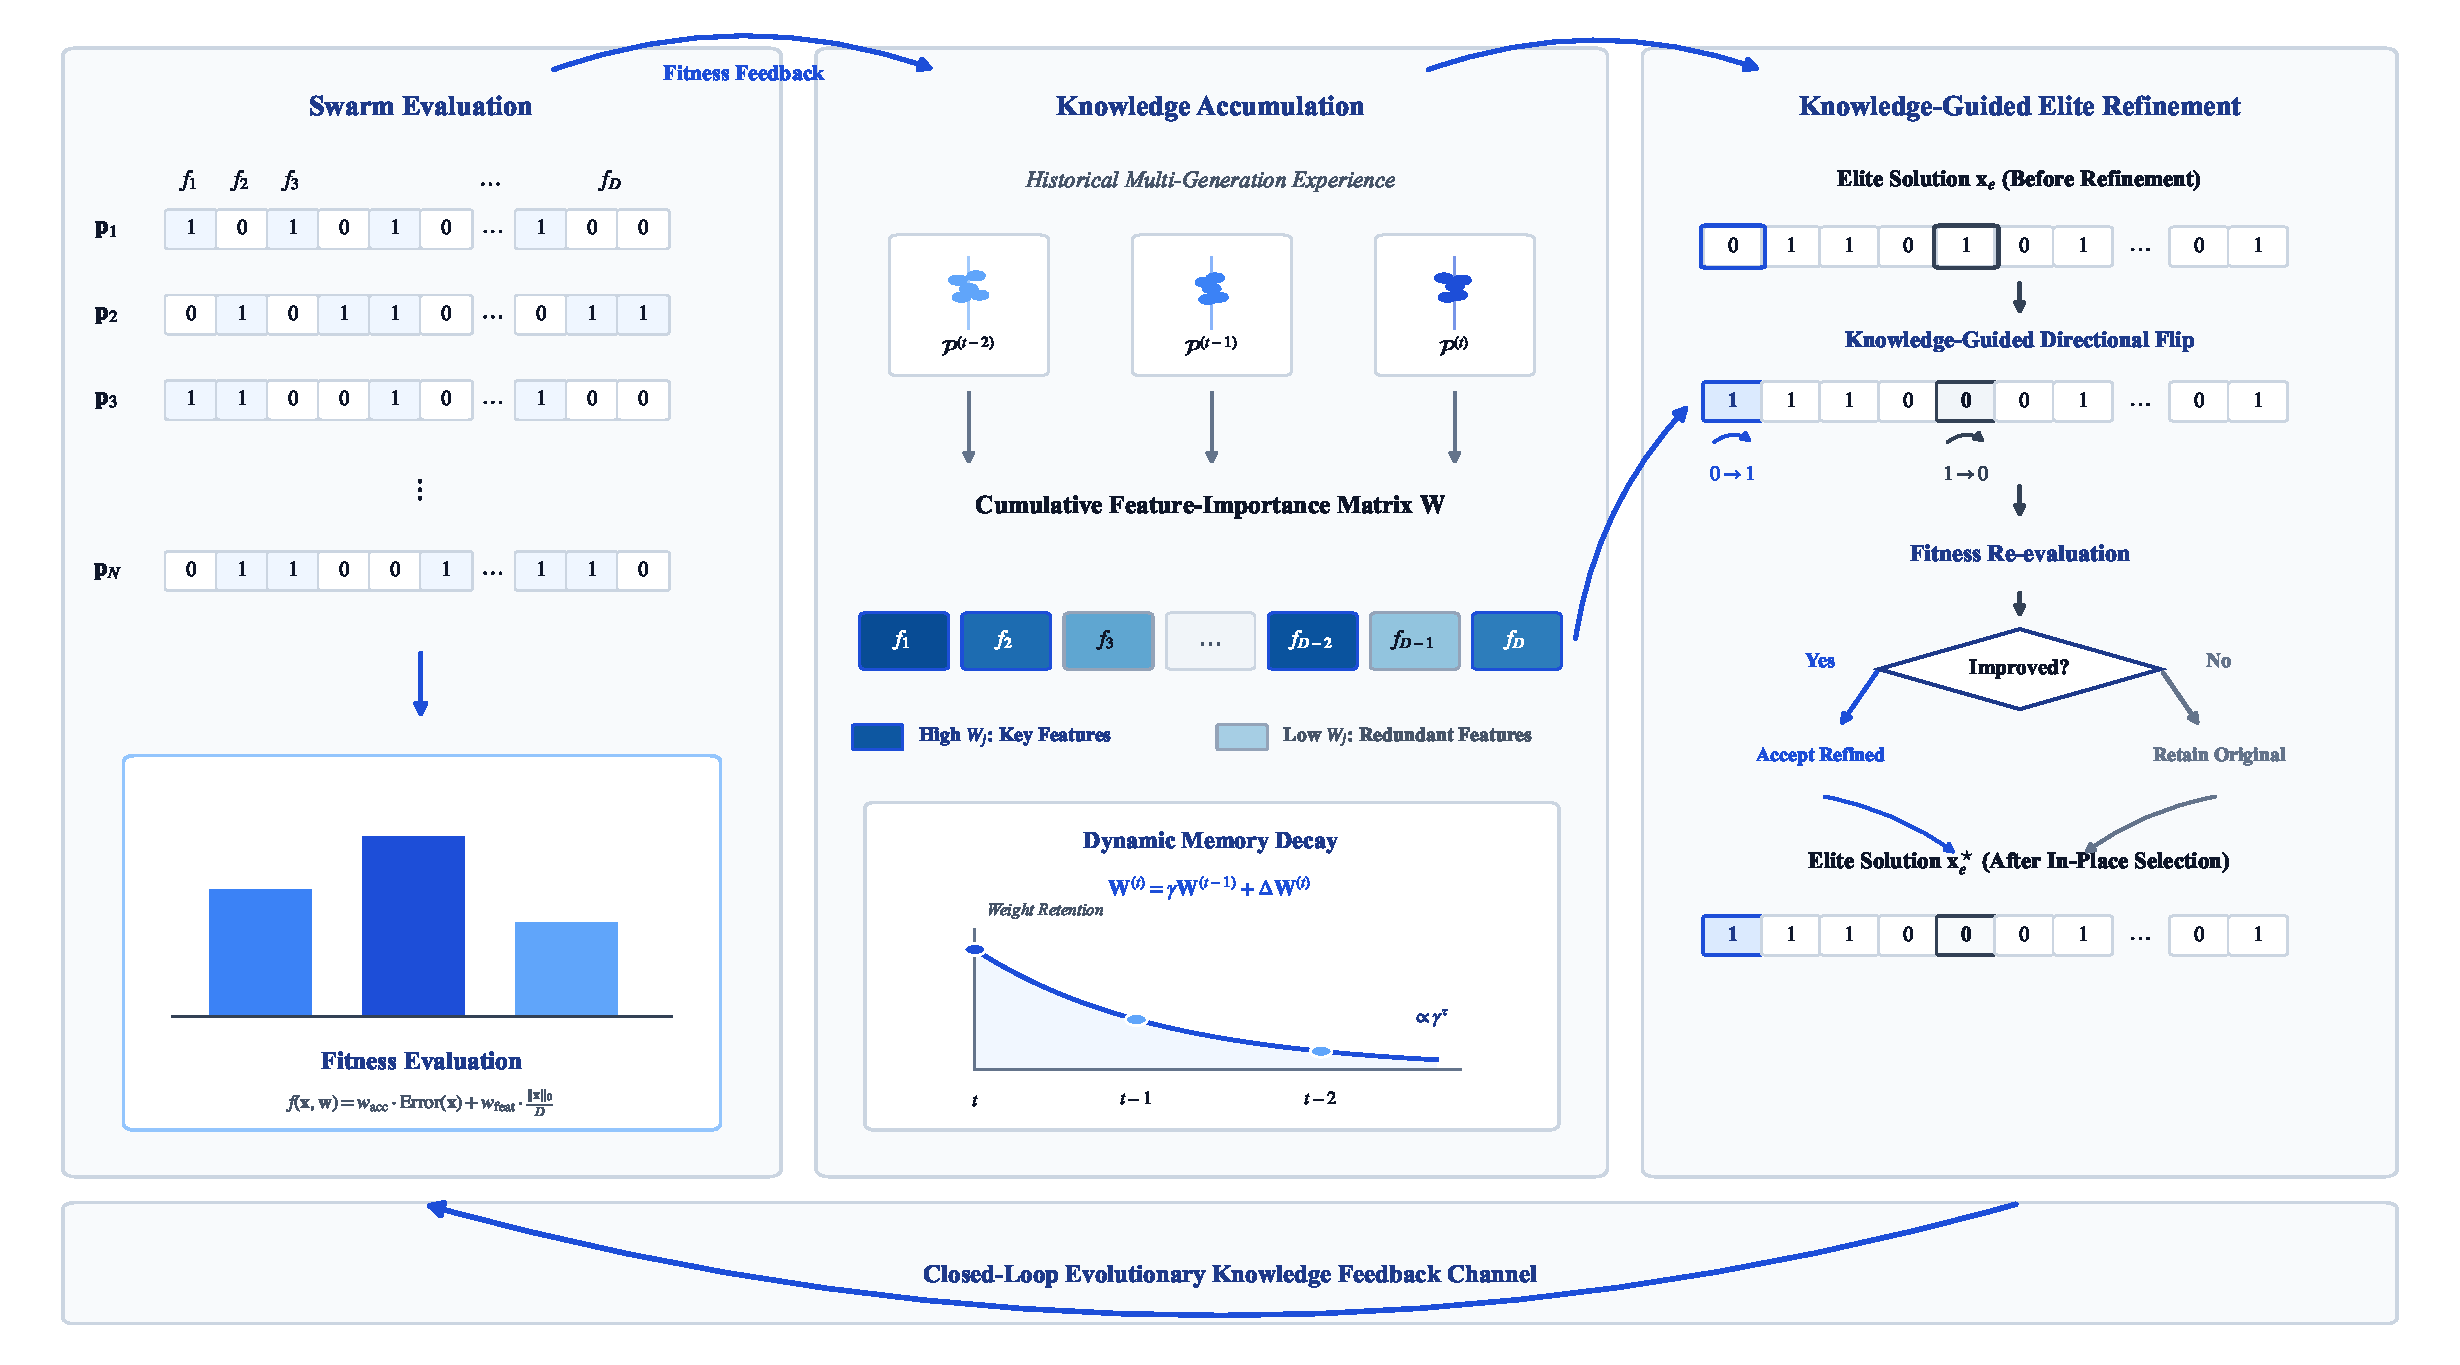
\includegraphics[width=0.95\linewidth]{F3_ker_strategy_journal.pdf}
\caption{Operational workflow of the Knowledge-guided Elite Refinement (KER) strategy: candidate elites undergo either knowledge-guided directional refinement ($p=0.90$) guided by cumulative matrix $W$ or ergodic random exploration ($p=0.10$), evaluated in a closed-loop and admitted via greedy 1-to-1 in-place replacement.}
\label{F3}
\end{figure*}

At each generation, the top $\mathrm{elite\_k} = 3$ individuals (ranked by current fitness) are selected for refinement. For each elite individual $\mathbf{x}_e \in \{0, 1\}^D$, KER executes a probabilistic dual-branch operation (Fig.~\ref{F3}):
\begin{enumerate}
    \item \textbf{Ergodic Random Exploration Branch (Probability $p_{\mathrm{rand}} = 0.10$)}: To guarantee search ergodicity and prevent irreversible bias toward early-accumulated matrix patterns, $\lfloor \phi D \rfloor$ features are selected uniformly at random and inverted:
    \begin{equation}
    x'_{e,j} \leftarrow 1 - x_{e,j}, \quad \forall j \in \mathcal{S}_{\mathrm{rand}}, \quad |\mathcal{S}_{\mathrm{rand}}| = \lfloor \phi D \rfloor,
    \label{eq:ker_rand}
    \end{equation}
    where $\phi = \mathrm{flip\_frac} = 0.01$ defines the refinement perturbation budget.
    \item \textbf{Knowledge-Guided Directional Refinement Branch (Probability $1 - p_{\mathrm{rand}} = 0.90$)}: Each feature $j \in \{1, \ldots, D\}$ is assigned a state-dependent directional flip score $\sigma_j$:
    \begin{equation}
    \sigma_j = \begin{cases}
    +W_j, & \text{if } x_{e,j} = 0 \quad \text{(reward activating absent high-importance features)},\\[2pt]
    -W_j, & \text{if } x_{e,j} = 1 \quad \text{(reward deactivating present low-importance features)}.
    \end{cases}
    \label{eq:flip_score}
    \end{equation}
    The scores can be written compactly as $\sigma_j = (1 - 2 x_{e,j}) \cdot W_j$. We identify the index set $\mathcal{S}_{\mathrm{know}}$ containing the $\lfloor \phi D \rfloor$ features possessing the highest flip scores $\sigma_j$:
    \begin{equation}
    \mathcal{S}_{\mathrm{know}} = \arg\max_{\substack{\mathcal{S} \subset \{1, \ldots, D\} \\ |\mathcal{S}| = \lfloor \phi D \rfloor}} \sum_{j \in \mathcal{S}} \sigma_j.
    \label{eq:top_scores}
    \end{equation}
    The directional refinement is then applied:
    \begin{equation}
    x'_{e,j} = \begin{cases}
    1 - x_{e,j}, & \text{if } j \in \mathcal{S}_{\mathrm{know}},\\[2pt]
    x_{e,j}, & \text{otherwise}.
    \end{cases}
    \label{eq:ker_flip}
    \end{equation}
\end{enumerate}

\subsubsection{1-to-1 In-Place Replacement and Bounded Evaluation Budget}

The perturbed offspring $\mathbf{x}'_e$ is evaluated under current objective weights $\mathbf{w}(t)$. A greedy \textbf{1-to-1 in-place replacement rule} is enforced:
\begin{equation}
\mathbf{x}_e^{\star} = \begin{cases}
\mathbf{x}'_e, & \text{if } f(\mathbf{x}'_e, \mathbf{w}(t)) < f(\mathbf{x}_e, \mathbf{w}(t)),\\[2pt]
\mathbf{x}_e, & \text{otherwise}.
\end{cases}
\label{eq:inplace}
\end{equation}
If improved, $\mathbf{x}'_e$ immediately overwrites $\mathbf{x}_e$ in the population and updates the global best if $f(\mathbf{x}'_e) < f_{\mathrm{gbest}}$.

\textbf{Rationale over $2N$-Candidate Pooling}: Unlike early multi-task prototypes that maintain an expanded $2N$ competitive selection pool, 1-to-1 in-place replacement incurs zero archive management overhead and prevents high selection pressure from prematurely collapsing population diversity.

\textbf{Bounded Refinement Budget}: Because $\mathrm{elite\_k} = 3$ is strictly fixed and $\phi = 0.01$ modifies only $1\%$ of the feature dimensions, KER executes within an exact bounded evaluation overhead of $k_e = 3$ function evaluations per generation, avoiding exponential computational expansion. Algorithm~\ref{alg:ker} details the KER operator.

\begin{algorithm}[!htb]
\caption{Knowledge-guided Elite Refinement (KER)}
\label{alg:ker}
\begin{algorithmic}[1]
\Require Elite candidate $\mathbf{x}_e$, importance matrix $W$, perturbation fraction $\phi=0.01$, random branch probability $p_{\mathrm{rand}}=0.10$, objective weights $\mathbf{w}(t)$
\Ensure Refined elite solution $\mathbf{x}_e^{\star}$ satisfying $f(\mathbf{x}_e^{\star}) \le f(\mathbf{x}_e)$
\State Sample random variable $r \sim \mathcal{U}(0, 1)$
\State $k_{\mathrm{flip}} \leftarrow \max(1, \lfloor \phi D \rfloor)$
\If{$r < p_{\mathrm{rand}}$} \Comment{10\% Ergodic random exploration branch}
    \State Sample subset $\mathcal{S}_{\mathrm{rand}} \subset \{1, \ldots, D\}$ uniformly at random with $|\mathcal{S}_{\mathrm{rand}}| = k_{\mathrm{flip}}$
    \State $\mathbf{x}'_e \leftarrow \mathbf{x}_e$; \quad $x'_{e,j} \leftarrow 1 - x_{e,j}, \; \forall j \in \mathcal{S}_{\mathrm{rand}}$
\Else \Comment{90\% Knowledge-guided directional refinement branch}
    \For{$j = 1$ \textbf{to} $D$}
        \State $\sigma_j \leftarrow (1 - 2 x_{e,j}) \cdot W_j$ \Comment{Compute directional score \eqref{eq:flip_score}}
    \EndFor
    \State Find subset $\mathcal{S}_{\mathrm{know}}$ of size $k_{\mathrm{flip}}$ with top $\sigma_j$ values \eqref{eq:top_scores}
    \State $\mathbf{x}'_e \leftarrow \mathbf{x}_e$; \quad $x'_{e,j} \leftarrow 1 - x_{e,j}, \; \forall j \in \mathcal{S}_{\mathrm{know}}$
\EndIf
\State Evaluate offspring fitness $f' \leftarrow f(\mathbf{x}'_e, \mathbf{w}(t))$ using \eqref{eq:fitness}
\If{$f' < f(\mathbf{x}_e, \mathbf{w}(t))$}
    \State $\mathbf{x}_e^{\star} \leftarrow \mathbf{x}'_e$ \Comment{In-place elite replacement \eqref{eq:inplace}}
\Else
    \State $\mathbf{x}_e^{\star} \leftarrow \mathbf{x}_e$
\EndIf
\State \Return $\mathbf{x}_e^{\star}$
\end{algorithmic}
\end{algorithm}

\subsection{Two-Phase Dynamic Objective Weight Scheduling Strategy}\label{sec:twophase}

\subsubsection{Deficiency Analysis and Design Rationale}

In multi-objective feature selection transformed via weighted-sum aggregation, conventional algorithms universally fix the objective weights throughout the entire evolutionary trajectory (e.g., static $\mathbf{w} = [0.90, 0.10]$)~\cite{miao2024,mel2024}. However, feature selection exhibits an intrinsic temporal asymmetry between early and late search stages:
\begin{itemize}
    \item \textbf{Early Evolutionary Stage}: The swarm navigates dense, highly noisy regions containing thousands of redundant features. The primary optimization objective is rapid, aggressive dimensionality reduction to prune non-informative search space.
    \item \textbf{Late Evolutionary Stage}: Once redundant features have been aggressively stripped and the swarm converges to a compact candidate set ($<100$ features), the objective shifts decisively toward fine-grained accuracy tuning among subtle biomarker combinations.
\end{itemize}
A static weight vector compromises between these competing stage-dependent goals, leading to sluggish early feature reduction and inadequate late-stage accuracy refinement.

\subsubsection{Dynamic Weight Scheduling Formulation}

\begin{figure*}[!htb]
\centering
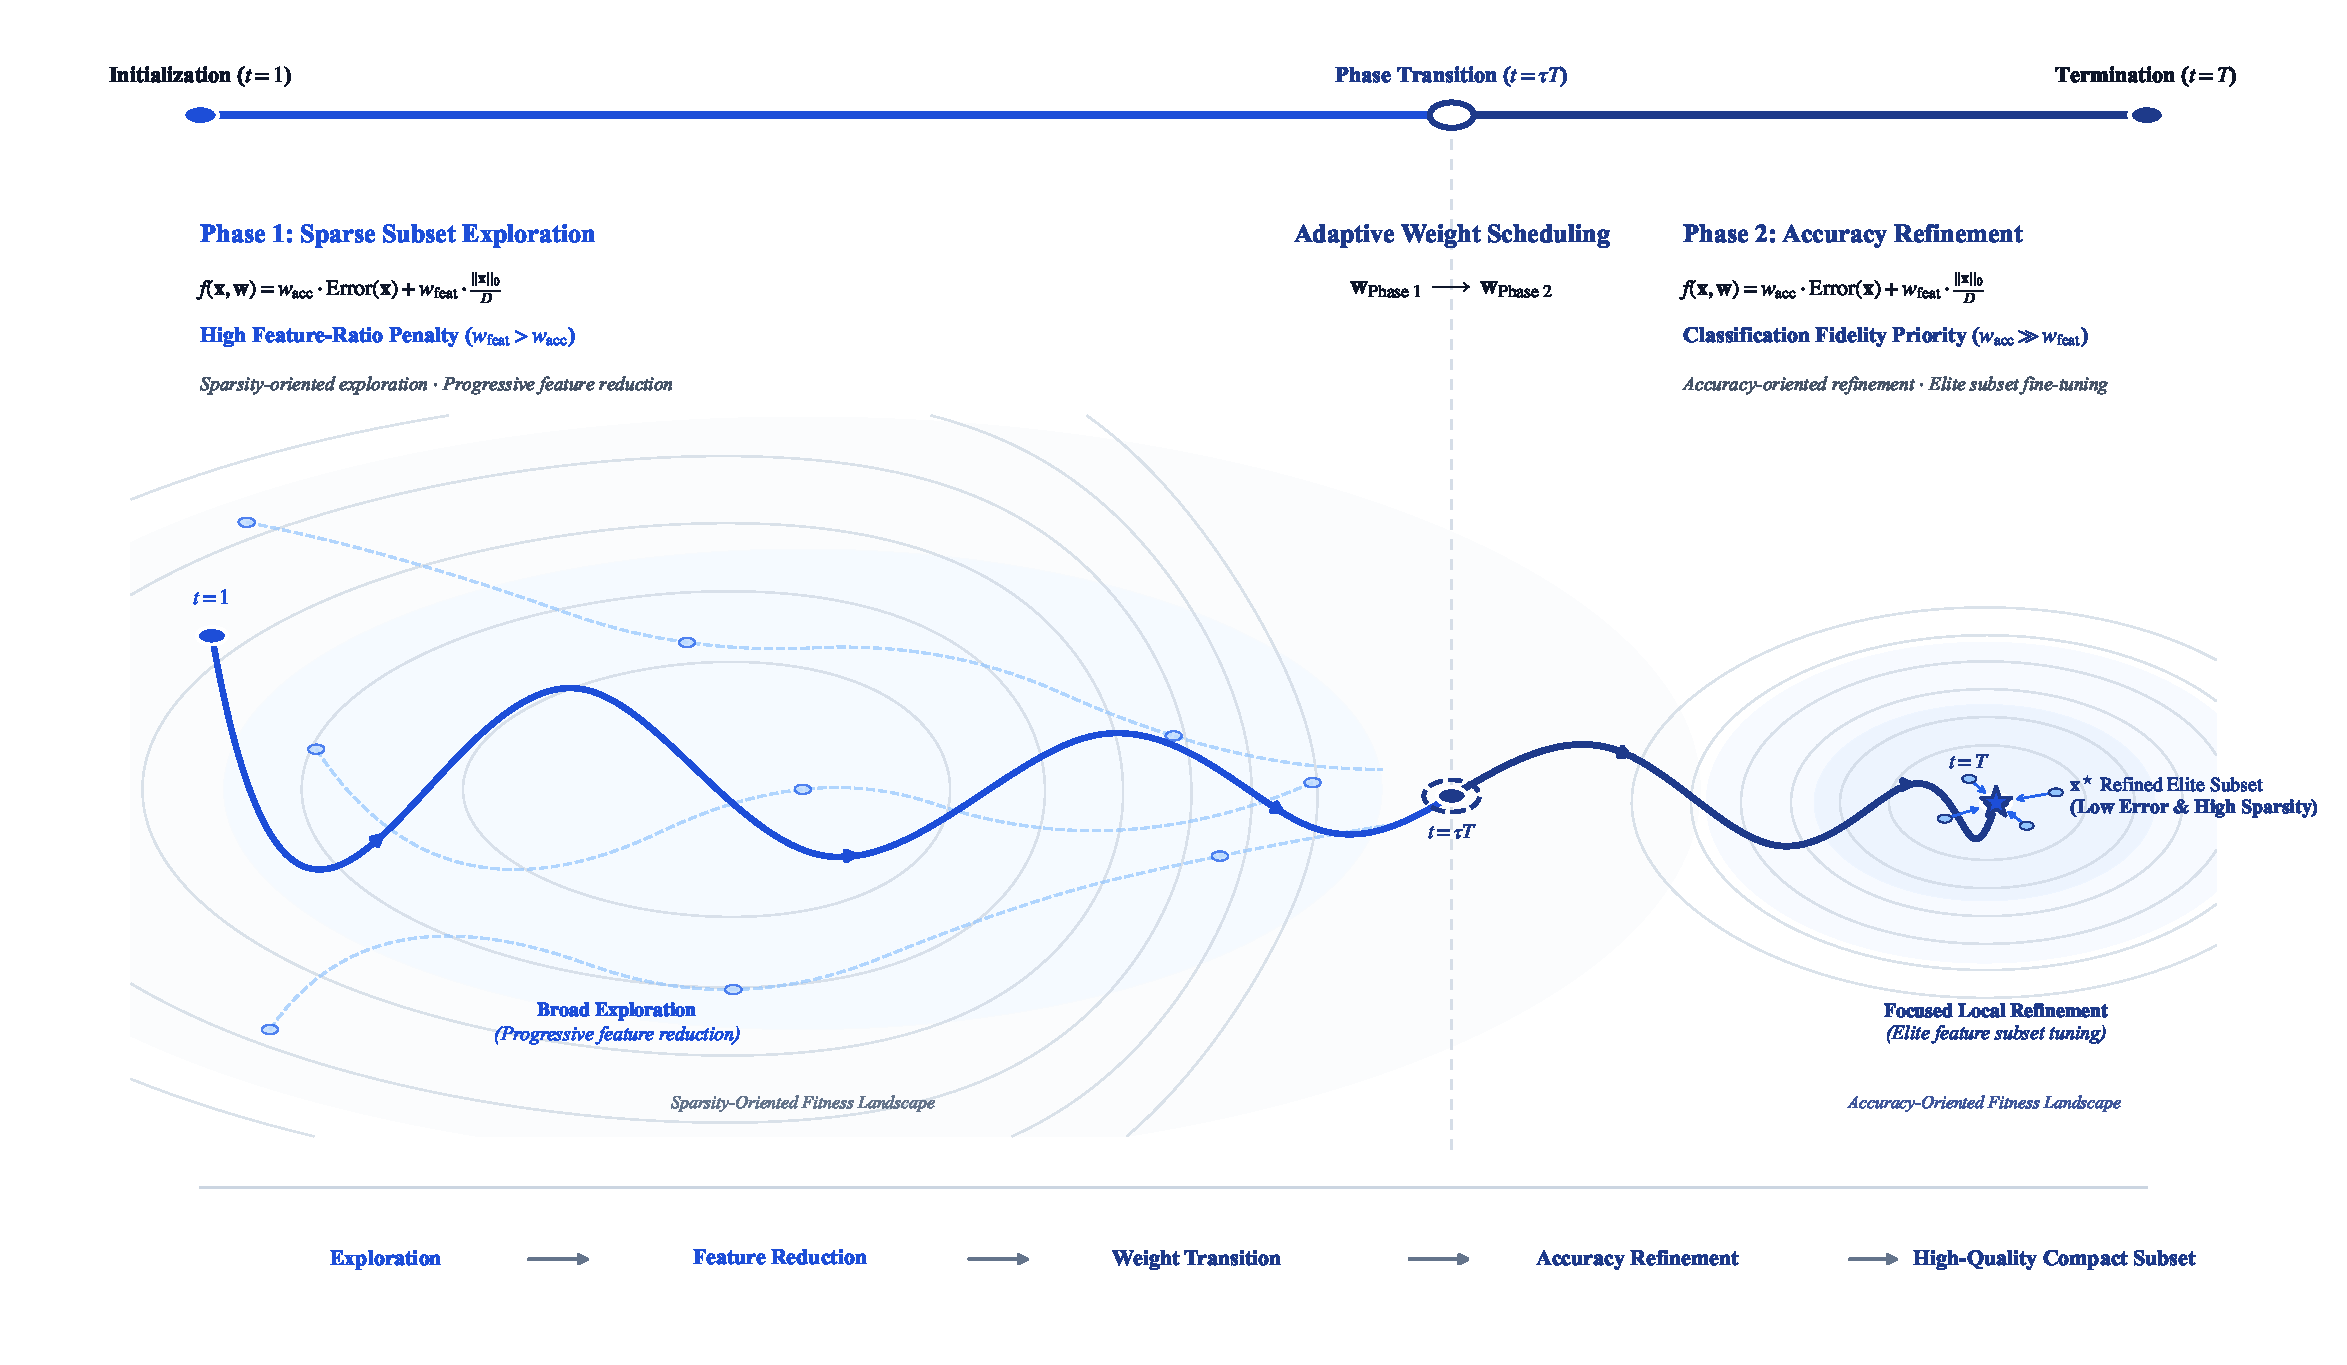
\includegraphics[width=0.95\linewidth]{F4_tps_strategy_journal.pdf}
\caption{Evolutionary optimization mechanism of the Two-Phase Dynamic Objective Weight Scheduling (TPS) strategy: across a continuous scalarized fitness landscape, search transitions at $t = 0.70\,T$ from Phase~1 ($(\alpha, \beta) = (0.70, 0.30)$, broad exploration and progressive feature reduction) to Phase~2 ($(\alpha, \beta) = (0.95, 0.05)$, focused accuracy refinement), ultimately converging to a high-quality compact feature subset.}
\label{F4}
\end{figure*}

To reconcile this temporal conflict, KDS-EL introduces the \textbf{Two-Phase Weight Scheduling (TPS)} strategy, as illustrated in Fig.~\ref{F4}. The total generational budget $T = 100$ is partitioned at split point $\alpha = \mathrm{PhaseSplit} = 0.70$. The dynamic dual-objective weight vector $\mathbf{w}(t) = [w_a(t), w_f(t)]$ is governed by a step-transition function:
\begin{equation}
\mathbf{w}(t) = \begin{cases}
[0.70, \; 0.30], & \text{for } 1 \le t \le \lfloor \alpha T \rfloor \quad \text{(Phase~1: Aggressive Feature Pruning)},\\[4pt]
[0.95, \; 0.05], & \text{for } \lfloor \alpha T \rfloor < t \le T \quad \text{(Phase~2: Accuracy Refinement)}.
\end{cases}
\label{eq:twophase}
\end{equation}

The unified scalar fitness $f(\mathbf{x}, \mathbf{w}(t))$ of a binary feature subset $\mathbf{x} \in \{0, 1\}^D$ at generation $t$ is formulated as:
\begin{equation}
f(\mathbf{x}, \mathbf{w}(t)) = w_a(t) \cdot \mathrm{Error}(\mathbf{x}) + w_f(t) \cdot \left(\frac{\|\mathbf{x}\|_0}{D}\right),
\label{eq:fitness}
\end{equation}
where $\mathrm{Error}(\mathbf{x}) = 1 - \mathrm{Acc}(\mathbf{x})$ denotes the 5-fold cross-validation classification error rate evaluated by a $k$-nearest neighbors ($k\text{-NN}, k=3$) classifier, and $\|\mathbf{x}\|_0 / D = \frac{1}{D}\sum_{j=1}^D x_j$ represents the normalized feature selection ratio ($\mathrm{FSR}$).

In Phase~1 ($t \le 70$), the heavy feature-ratio penalty ($w_f = 0.30$) drives rapid elimination of thousands of non-informative features without sacrificing classification fidelity. In Phase~2 ($t > 70$), the weight switches to prioritize classification accuracy ($w_a = 0.95$), allowing the swarm and the KER operator to fine-tune delicate biomarker interactions over the surviving compact subspace. Algorithm~\ref{alg:twophase} specifies the TPS scheduling function.

\begin{algorithm}[!htb]
\caption{Two-Phase Dynamic Weight Scheduling}
\label{alg:twophase}
\begin{algorithmic}[1]
\Require Current generation $t$, maximum generations $T=100$, phase split ratio $\alpha=0.70$
\Ensure Dynamic dual-objective weight vector $\mathbf{w}(t) = [w_a(t), w_f(t)]$
\If{$t \le \lfloor \alpha \cdot T \rfloor$}
    \State $\mathbf{w}(t) \leftarrow [0.70, \; 0.30]$ \Comment{Phase 1: Coarse feature pruning}
\Else
    \State $\mathbf{w}(t) \leftarrow [0.95, \; 0.05]$ \Comment{Phase 2: Fine accuracy refinement}
\EndIf
\State \Return $\mathbf{w}(t)$
\end{algorithmic}
\end{algorithm}

\subsection{Integrated KDS-EL Main Algorithm}\label{sec:main_algo}

Algorithm~\ref{alg:kds_el} consolidates the holistic execution workflow of KDS-EL, integrating filter-based MI ranking, hybrid seeding, the two-phase evolutionary loop, cumulative importance matrix updating, and knowledge-guided elite refinement into a unified procedure.

\begin{algorithm}[!htb]
\caption{Complete Execution Workflow of KDS-EL}
\label{alg:kds_el}
\begin{algorithmic}[1]
\Require Dataset $\mathcal{D}=(X, Y)$ with $D$ features, population size $N=20$, maximum iterations $T=100$, split ratio $\alpha=0.70$, binarization threshold $\theta=0.60$, MI ratio $\rho=0.50$, decay $\gamma=0.99$, elite count $k_e=3$, flip fraction $\phi=0.01$, random branch probability $p_{\mathrm{rand}}=0.10$, stall patience $\tau=20$
\Ensure Optimal binary feature subset $\mathbf{x}^{\star} \in \{0, 1\}^D$
\State \textbf{/* Stage 1: Filter-level Feature Ranking */}
\State Compute mutual information $I(f_j; Y)$ for all $j \in \{1, \ldots, D\}$ via \eqref{eq:mi_def}
\State Normalize MI scores to construct relevance vector $\mathbf{m} \in [0, 1]^D$ via \eqref{eq:mi_norm}
\State \textbf{/* Stage 2: Knowledge-Guided Population Seeding */}
\State Initialize population $\{\mathbf{x}_i, \mathbf{p}_i\}_{i=1}^N$ via Algorithm~\ref{alg:mi_init} (MI-guided hybrid seeding)
\State Initialize cumulative feature-importance matrix $W \leftarrow \mathbf{0} \in \mathbb{R}^D$
\State Evaluate initial fitness $\{f_i\}_{i=1}^N$ under $\mathbf{w}(1) = [0.70, 0.30]$ via \eqref{eq:fitness}
\State Initialize personal bests: $\mathbf{p}_{\mathrm{best},i} \leftarrow \mathbf{x}_i, \; f_i^{\mathrm{pbest}} \leftarrow f_i, \; \forall i \in \{1, \ldots, N\}$
\State Identify global best: $\mathbf{g}_{\mathrm{best}} \leftarrow \arg\min_{\mathbf{p}_{\mathrm{best},i}} f_i^{\mathrm{pbest}}, \; f_{\mathrm{gbest}} \leftarrow \min f_i^{\mathrm{pbest}}$
\State Initialize stagnation counter $\mathrm{stall\_count} \leftarrow 0$
\State \textbf{/* Stage 3: Two-Phase Evolutionary Main Loop */}
\For{$t = 1$ \textbf{to} $T$}
    \State Update objective weights $\mathbf{w}(t) \leftarrow \text{Algorithm~\ref{alg:twophase}}(t, T, \alpha)$
    \State \textbf{/* Subpopulation 1: Inter-Task Velocity-Position Update */}
    \For{$i = 1$ \textbf{to} $N/2$}
        \State Update continuous velocity $\mathbf{v}_i$ and position $\mathbf{p}_i$ using PSO rules with Subpopulation 2 attractor
        \State Binarize position: $x_{i,j} \leftarrow \mathbb{I}(p_{i,j} \ge \theta), \; \forall j \in \{1, \ldots, D\}$
    \EndFor
    \State \textbf{/* Subpopulation 2: Importance-Guided Feature Sampling */}
    \For{$i = N/2 + 1$ \textbf{to} $N$}
        \State Sample binary features based on cumulative matrix $W$ and personal best $\mathbf{p}_{\mathrm{best},i}$
    \EndFor
    \State \textbf{/* Fitness Evaluation and Importance Matrix Harvesting */}
    \For{$i = 1$ \textbf{to} $N$}
        \State Evaluate candidate fitness $f_i \leftarrow f(\mathbf{x}_i, \mathbf{w}(t))$ using \eqref{eq:fitness}
    \EndFor
    \State Update and discount importance matrix $W \leftarrow \text{Algorithm~\ref{alg:importance_update}}(\{\mathbf{x}_i\}, \{\mathbf{p}_{\mathrm{best},i}\}, \{f_i\}, \{f_i^{\mathrm{pbest}}\}, W, \gamma)$
    \State Update personal bests: if $f_i < f_i^{\mathrm{pbest}}$ then $\mathbf{p}_{\mathrm{best},i} \leftarrow \mathbf{x}_i, \; f_i^{\mathrm{pbest}} \leftarrow f_i$
    \State \textbf{/* Stage 4: Knowledge-Guided Elite Refinement */}
    \State Identify top $k_e$ elite indices $\mathcal{E} \subset \{1, \ldots, N\}$ based on $f_i^{\mathrm{pbest}}$
    \For{\textbf{each} $e \in \mathcal{E}$}
        \State $\mathbf{p}_{\mathrm{best},e} \leftarrow \text{Algorithm~\ref{alg:ker}}(\mathbf{p}_{\mathrm{best},e}, W, \phi, p_{\mathrm{rand}}, \mathbf{w}(t))$ \Comment{1-to-1 in-place refinement}
    \EndFor
    \State \textbf{/* Global Best Update and Stagnation Check */}
    \State Find current best $\mathbf{x}_{\mathrm{curr}} \leftarrow \arg\min_{\mathbf{p}_{\mathrm{best},i}} f_i^{\mathrm{pbest}}$ with fitness $f_{\mathrm{curr}}$
    \If{$f_{\mathrm{curr}} < f_{\mathrm{gbest}}$}
        \State $\mathbf{g}_{\mathrm{best}} \leftarrow \mathbf{x}_{\mathrm{curr}}, \; f_{\mathrm{gbest}} \leftarrow f_{\mathrm{curr}}, \; \mathrm{stall\_count} \leftarrow 0$
    \Else
        \State $\mathrm{stall\_count} \leftarrow \mathrm{stall\_count} + 1$
    \EndIf
    \If{$\mathrm{stall\_count} \ge \tau$}
        \State Execute adaptive re-initialization via Algorithm~\ref{alg:mi_reinit}
        \State $\mathrm{stall\_count} \leftarrow 0$
    \EndIf
\EndFor
\State \Return $\mathbf{x}^{\star} \leftarrow \mathbf{g}_{\mathrm{best}}$
\end{algorithmic}
\end{algorithm}

\subsection{Asymptotic Computational and Space Complexity Analysis}\label{sec:complexity}

To establish the computational efficiency of KDS-EL, we conduct a rigorous asymptotic complexity analysis covering all algorithmic components.

\subsubsection{Time Complexity Decomposition}

The execution time of KDS-EL is decomposed into two distinct phases:
\begin{enumerate}
    \item \textbf{Offline Preprocessing Phase (Mutual Information Calculation)}:
    Computing the mutual information $I(f_j; Y)$ between each feature $f_j$ and class label $Y$ requires $O(N_{\mathrm{samp}})$ operations per feature, where $N_{\mathrm{samp}}$ is the number of training samples. For all $D$ features, computing and sorting the baseline MI vector incurs:
    \begin{equation}
    T_{\mathrm{pre}} = O(D \cdot N_{\mathrm{samp}} + D \log D).
    \label{eq:t_pre}
    \end{equation}
    Because this step is executed only once prior to the evolutionary loop, its overhead is entirely negligible relative to iterative wrapper evaluations.
    \item \textbf{Iterative Evolutionary Main Loop ($T$ Iterations)}:
    In each of the $T$ generations, computational costs arise from four operations:
    \begin{itemize}
        \item \textit{Subpopulation Position Updates}: Updating particle velocities and continuous positions across the population of size $N$ incurs $O(N \cdot D)$ arithmetic operations.
        \item \textit{Fitness Wrapper Evaluation}: Evaluating the 5-fold cross-validation $k\text{-NN}$ classification accuracy for $N$ candidate particles requires:
        \begin{equation}
        T_{\mathrm{eval}} = O(N \cdot N_{\mathrm{samp}}^2 \cdot d_{\mathrm{selected}}),
        \label{eq:t_eval}
        \end{equation}
        where $d_{\mathrm{selected}} = \|\mathbf{x}\|_0$ is the number of active features in candidate $\mathbf{x}$.
        \item \textit{Importance Matrix Differential Updating and Decay}: Scanning changed features for improving particles and performing scalar decay across matrix $W$ incurs $O(N \cdot D + D)$ operations.
        \item \textit{Knowledge-Guided Elite Refinement (KER)}: Computing flip scores $\sigma_j$ for $k_e$ elites, selecting the top $\lfloor \phi D \rfloor$ features, flipping bits, and re-evaluating the $k_e$ refined elites requires $O(k_e \cdot (D + T_{\mathrm{eval\_single}}))$, where $T_{\mathrm{eval\_single}} = O(N_{\mathrm{samp}}^2 \cdot d_{\mathrm{selected}})$.
        \item \textit{Adaptive Stagnation Re-initialization}: When triggered (at most $\lfloor T/\tau \rfloor$ times), re-seeding and evaluating $N/2$ particles requires $O(\frac{N}{2} \cdot (D + T_{\mathrm{eval\_single}}))$.
    \end{itemize}
\end{enumerate}

Summing these terms across $T$ generations yields the total asymptotic time complexity:
\begin{equation}
\mathcal{T}_{\mathrm{total}} = O\Bigl(D \log D + T \cdot \bigl[N \cdot D + (N + k_e) \cdot N_{\mathrm{samp}}^2 \cdot d_{\mathrm{selected}}\bigr]\Bigr).
\label{eq:total_complexity}
\end{equation}

\subsubsection{Theoretical Complexity Equivalence and Practical Acceleration}

Because $k_e = 3 \ll N = 20$ and $N_{\mathrm{samp}}^2 \cdot d_{\mathrm{selected}} \gg D$, the dominant asymptotic per-generation complexity of KDS-EL is strictly governed by wrapper evaluations:
\begin{equation}
\mathcal{T}_{\mathrm{KDS-EL}} = O(T \cdot N \cdot N_{\mathrm{samp}}^2 \cdot d_{\mathrm{selected}}),
\label{eq:dominant_complexity}
\end{equation}
which is identically of the same asymptotic order as the baseline MEL~\cite{mel2024} ($O(T \cdot N \cdot N_{\mathrm{samp}}^2 \cdot d_{\mathrm{MEL}})$).

Crucially, in the baseline MEL, random initialization and sluggish feature reduction result in dense candidate subsets ($d_{\mathrm{MEL}} \approx 2{,}722$ active features on average). In contrast, KDS-EL's MI seeding and Phase~1 aggressive feature pruning rapidly compress the active feature count to $d_{\mathrm{KDS-EL}} \approx 88$ features. Because $k\text{-NN}$ distance calculation scales linearly with $d_{\mathrm{selected}}$, evaluating a KDS-EL particle is over an order of magnitude faster than evaluating an unpruned MEL particle. Consequently, KDS-EL delivers a dramatic \textbf{3.4$\times$ empirical wall-clock speedup} (51.4~s vs.\ 175.0~s) while incorporating richer knowledge operators.

\subsubsection{Space Complexity}

The memory footprint of KDS-EL comprises: (i) the population continuous and binary position matrices ($O(N \cdot D)$), (ii) personal-best vectors ($O(N \cdot D)$), (iii) the cumulative feature-importance matrix $W$ ($O(D)$), and (iv) the precomputed normalized MI vector $\mathbf{m}$ ($O(D)$). The overall space complexity is:
\begin{equation}
\mathcal{S}_{\mathrm{total}} = O(N \cdot D + N_{\mathrm{samp}} \cdot D),
\label{eq:space_complexity}
\end{equation}
which scales strictly linearly with dimension $D$, ensuring minimal memory consumption.

